\section{Verziókövetés és projektmenedzsment}
A rendszer fejlesztéséhez szükséges volt egy verziókövető rendszert választani. Erre azért volt szükség, mivel ketten készítettük a projektet, a verziókövető rendszer segítséget nyújtott, a sikeres közös fejlesztéshez. A verziókövető rendszer mellett egy projekt menedzsment eszközt is választottunk, ahol a feladatainkat (task) tudtuk nyilvántartani.
\subsection{Bitbucket}
Kódverzió követő rendszer \cite{bitbucket}, amelyet a fejlesztők számára hoztak létre. Lehetőséget biztosít a git adattárak kezeléséhez és a fejlesztési folyamat végigvezetéséhez. 

A \ref{fig:bitbu} ábrán látható, a projekt kommitolásnak visszakövetése, oldalból meg, hogy még milyen opciókkal rendelkezünk, például: ha rálépünk a Source opcióra eljön a forráskódunknak az utolsó verziója. Tulajdonképpen nyomon követhetjük a közös fejlesztés lépéseit, visszanézhetjük a kódon történt változtatásokat és egy biztonságos helyen tárolhatjuk a projekt forrás kódját.
\begin{figure}[H]
	\centering
	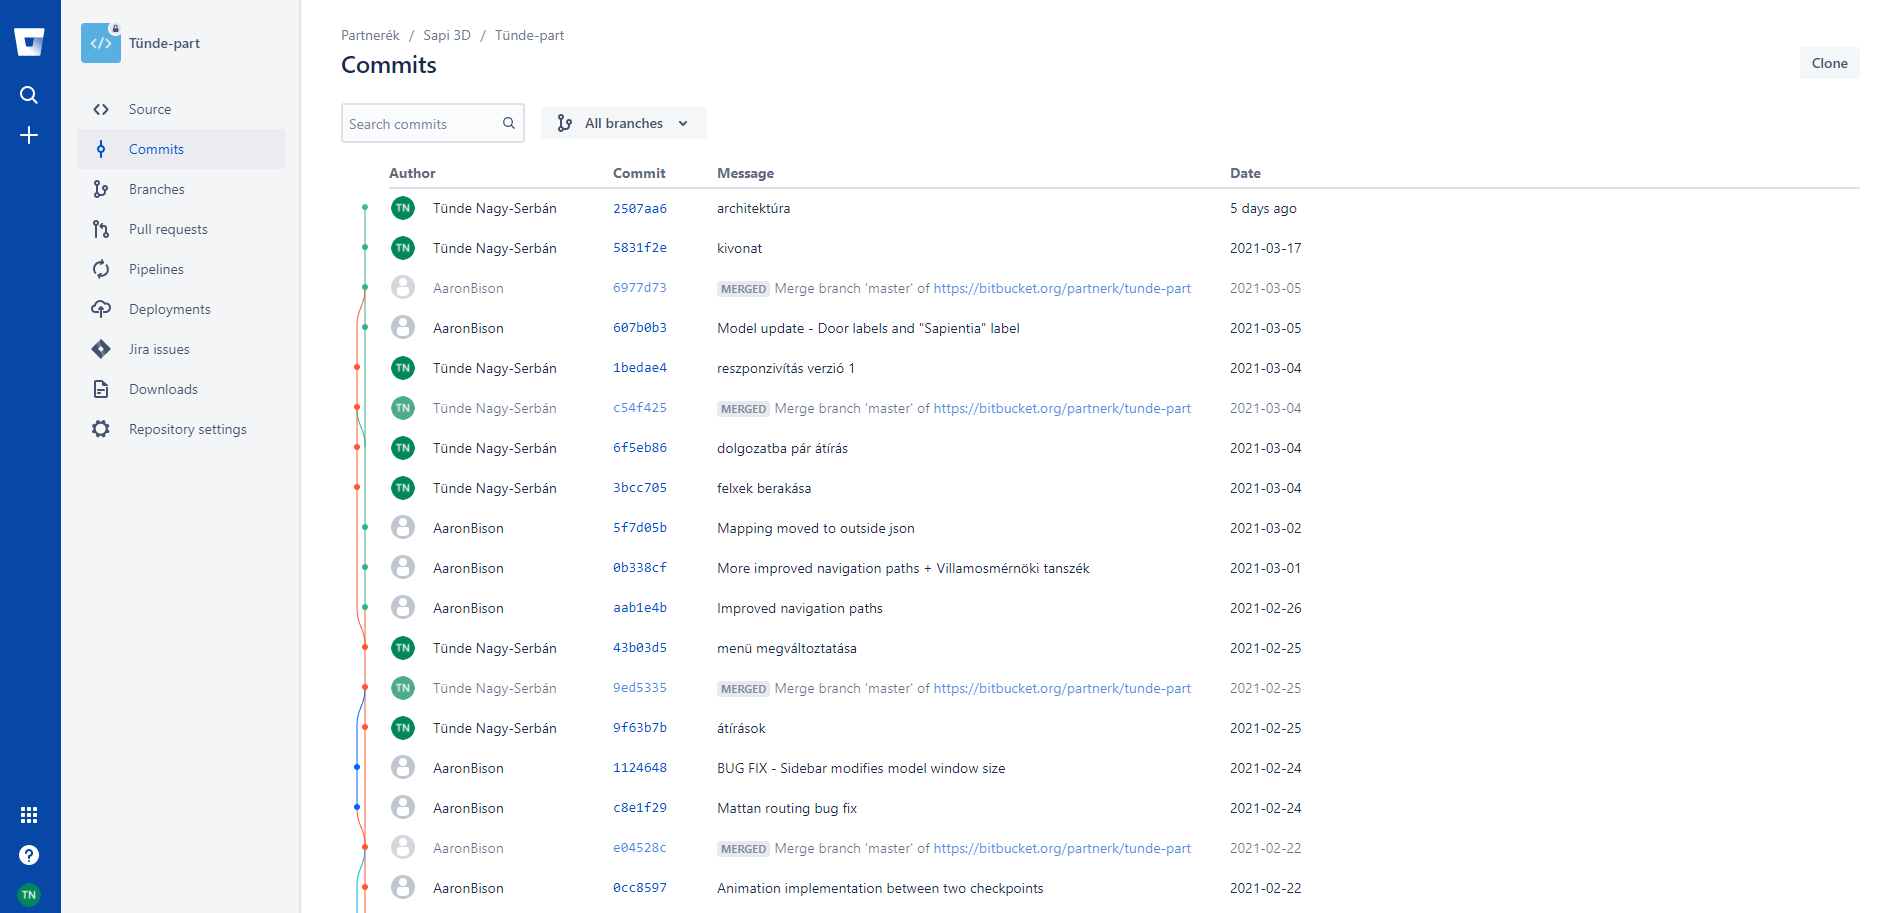
\includegraphics[width=0.8\linewidth]{figures/images/bitbucket.png}
	\caption[Példa a Bitbucket verzió követésére]{\textit{Példa a Bitbucket verzió követésére}}
	\label{fig:bitbu}
\end{figure}
\subsection{Trello}
A Trello projektmenedzsment eszköz \cite{trello}, amely a projekteket különböző táblákba rendezi. A \ref{fig:trello} ábrán látható a saját projektmanadzselésünk. Megfigyelhetőek a különböző oszlopok, amelyekben láthatunk kissebb feladatokat. 

Az eszköz a {\textit{Kanban módszer}\footnotemark} alapján a feladat folyamatát jelzi, mint például a To-Do oszlop jelenti azokat a feladatokat amelyeket még el sem kezdtek a fejlesztők. A Progress oszlop jelzi, hogy mely feladatokon dolgoznak a fejlesztők. A Done oszlop jelzi, hogy mely feladatok lettek elvégezve. A fejlesztők eltudják látni a feladatokat egy-egy színnel is, amely jelzi a többi fejlesztőnek, hogy azt a feladatot ki végzi. A feladatokat lehet mozgatni állapotuktól függően.
\footnotetext{https://promanconsulting.hu/kanban-rendszer/}

Egy jó tulajdonsága a Trellonak, hogy össze lehet kötni a Bitbucket-tel így nem kell külön megnyítani a két felületet, hanem egy felület alatt meglehet nézni mindkettőt. 
\begin{figure}[H]
	\centering
	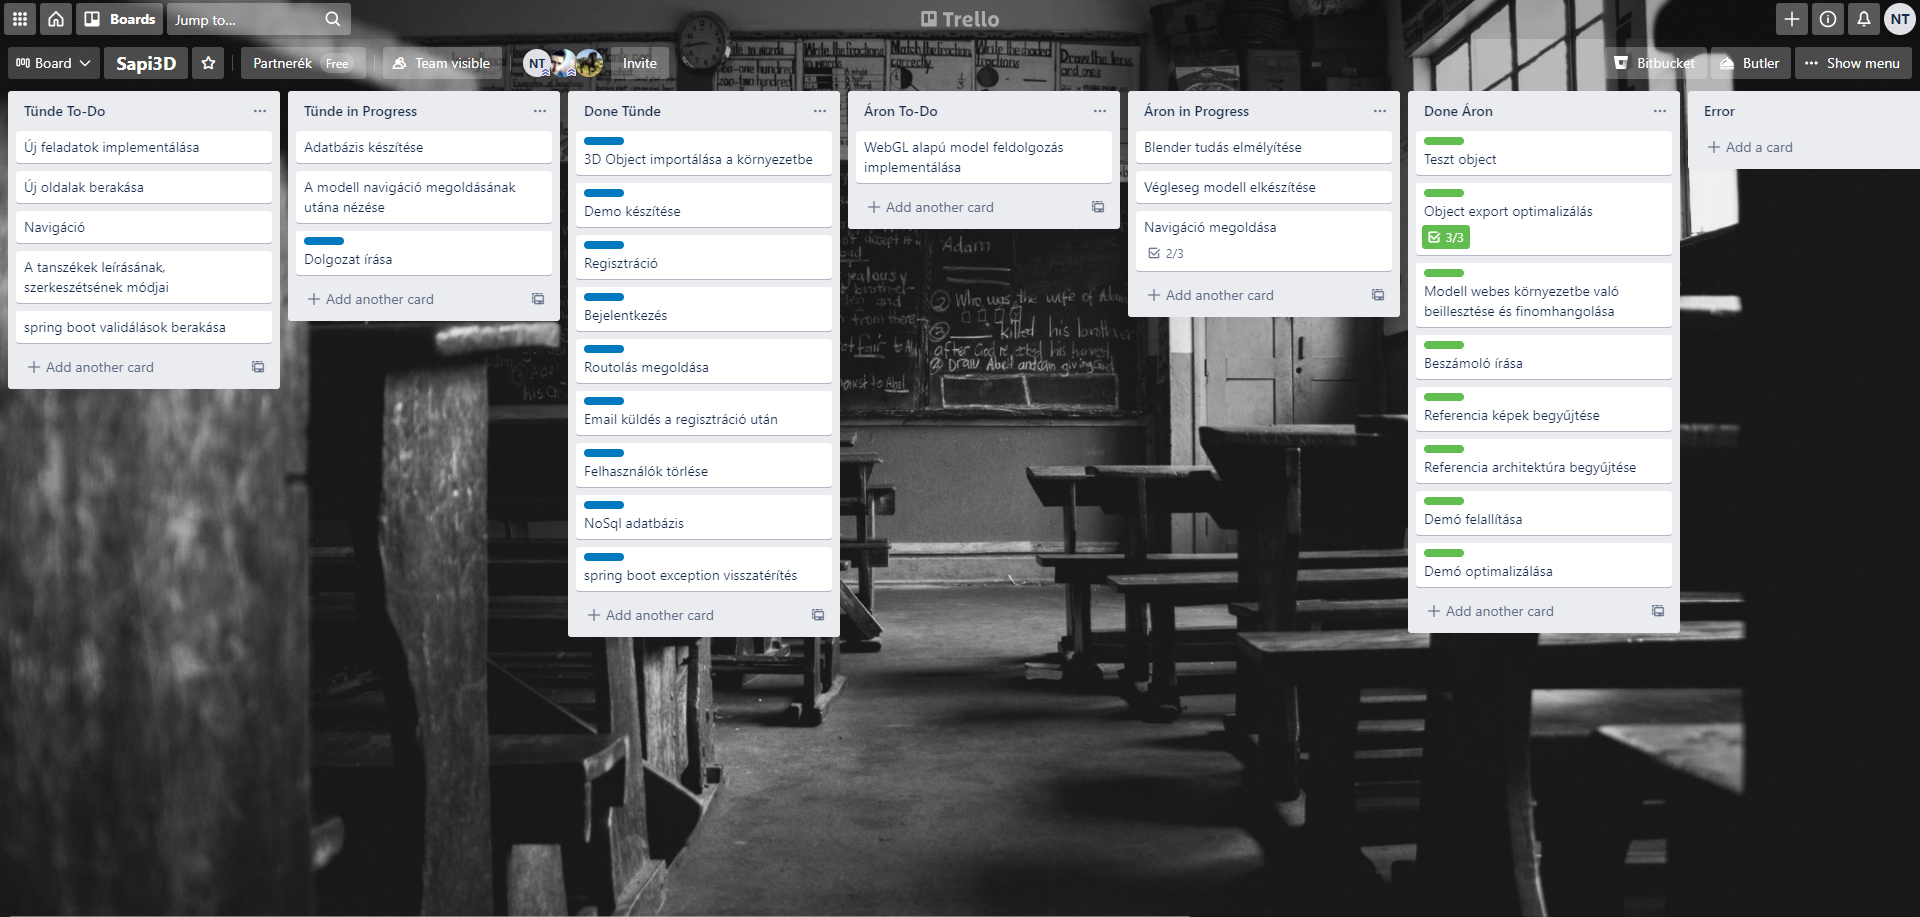
\includegraphics[width=1\linewidth]{figures/images/trello.png}
	\caption[Példa a Trello projekt menedzsment eszközre]{\textit{Példa a Trello projekt menedzsment eszközre}}
	\label{fig:trello}
\end{figure}
